\documentclass{ltjarticle}
\usepackage{geometry}
\usepackage[dvipdfmx]{graphicx}
\usepackage[colorlinks=true, allcolors=blue] {hyperref}
\usepackage{amsmath}
\usepackage{mathtools}
% ページの余白を1.25インチにする
\geometry{
    left=1.25truein,
    right=1.25truein,
    top=1.25truein,
    bottom=1.25truein,
}

\begin{document}
\begin{titlepage}
    \begin{center}
        {\Large 令和5年}
        \vspace{10truept}

        {\Large 修士論文草稿}
        \vspace*{180truept}

        {\Huge タイトル} 
        \vspace{160truept}

        {\Large 指導教員:相馬 隆郎}
        \vspace{30truept}

        {\Large 東京都立大学大学院}
        \vspace{10truept}

        {\Large 電子情報システム工学域}
        \vspace{30truept}

        {\Large 学修番号:22861651}
        \vspace{10truept}
        
        {\Large 氏名:西原涼介}
    \end{center}
\end{titlepage}
\noindent
{\LARGE 論文要旨}
\vspace{20truept}

ここから論文要旨

% 目次
\newpage
\tableofcontents
\clearpage

\part{はじめに}
\vspace{10truept}
\section{研究背景}
近年, Amazonや楽天市場などの大手ECサイトをはじめ、数多くのECサイトが普及し,  その利用者も急増して
いる. そして, 商品を購入する際にECサイトのレビューを参考にしている利用者の割合は約70\%と言われていて, そ
の中でもレビューの信頼性を重要視している人が多いことが明らかになっている. また, 多くの企業にとって, ECサイトの
レビューからユーザーの嗜好や意見を分析し,マーケティングに活用することが重要な課題となっている.そのため,
ECサイトのレビューの信頼性や参考になるかどうかを評価する評判分析や口コミ分析, レビューを様々なトピックに分類する文書分類に関する
研究が多く行われている. 例えば, 関連研究の項で詳しく紹介する「機械学習を用いた自然言語処理による商品レビューの評価」[1]では, Amazonの商品レビュー
を機械学習を用いて参考になる順に並びかえるシステムの構築, 及びその評価に関する研究を行っている。
また近年では, 従来のECサイトや商品のWebページ以外にも, YouTubeのような
動画投稿サイトやX(旧Twitter)やInstagramなどのSNSで自社製品・サービスの宣伝を行う企業が増えてきている. 
それにつれて, 商品を購入する際にSNSやYouTube上でその商品を宣伝している投稿を参考にしている人も増加している. 
そのため, SNSやYouTube上の広告に対するユーザーのコメントも, 他のユーザーが商品の購入を検討する際の重要な判断
材料になり得ると考えられる. つまり, SNSやYouTube上での商品の宣伝に対するコメントは, ECサイトのレビュー
と同等の機能を持ち, その信頼性や参考になるかどうかが重要になるため, 
評判分析や文書分類の研究の対象になると考えられる. ここで, SNSやYouTubeは商品レビューのページとは異なり, 
誰でも気軽にコメントを投稿できたり, その投稿内容も自由という特性上, 商品やサービスに関係ないコメントが
多数存在する.

そこで, 本研究では分析対象をYouTube上で自社製品やサービスを宣伝している動画に対するユーザーのコメントとし, 
トピックモデルの一種であるBiterm Topic Modelによる商品に関するトピック抽出を用いて, 
その動画に対するユーザーのコメントから, 宣伝している商品やサービスに対して関連性が高いコメントを
抽出するシステムの作成, 及び作成したシステムの人手に対する精度の検証を行った. 

本論文の第Ⅰ部では, ECサイトのレビューにおける評判分析やトピックモデルを用いた文書分類に関する関連研究の紹介, 
また本研究の研究目的を明確に説明する.
第Ⅱ部では, 本研究で用いる二つのトピックモデルの説明, 及び提案手法のシステムや実装方法について説明する.
第Ⅲ部では, 実際のYouTube上の動画に対するコメントを用いた実験結果を述べる.
第Ⅳ部では, 実験結果をもとに考察した提案手法の有効性や将来性について述べる. 

\newpage
\section{関連研究}
本研究を進めるにあたり, 研究テーマの方向性決めや研究課題の発見, 及び本研究で用いている技術に関して参考にした
論文を4つ紹介する. 
\subsection{機械学習を用いた自然言語処理による商品レビューの評価[1]}
この論文では, ユーザーが商品レビューを読んで参考になったかどうかを評価する機能が備わっていない
ECサイトの場合に, 数多くあるレビューから参考になる情報を探す必要がある問題に着目し, 
機械学習を用いた自然言語処理の手法で分析, 評価を行い, レビューを参考になる順番に並び替える
システムの構築を目的としている. そして並び替えた順番が正しいかどうかを評価するために, クイックソートを利用した
新しい評価法であるQE法を提案している. 

図\ref{fig:関連研究1システム概要図}はこの論文で提案されている, レビューを参考になる順番に並び替えるシステムの概要図である. はじめに, 
インターネット経由でAmazonの商品レビューのデータ取得し, 学習用データと評価データに分ける. 学習段階では, レビュー文章の
正規化や各前処理を施し, 教師データとして準備する. 
この研究では, 全角数字やアルファベットを半角に変換したり, 
数字は全て0に置換, アルファベットは全て小文字に変換などの正規化を行っている. また, 日本語形態素解析システムであるMeCab
を用いて形態素解析を行い, 品詞ごとに``\_''で分割する. その後, 活用語の原型への変換, 及びストップワード除去を行っている.
例えば, 「ロボットは24時間働けるのでAIに仕事をとられる.」という文章の場合, 正規化と前処理を施すことで, 
「ロボット\_0\_働ける\_ai\_仕事\_とる.」となる. この一連の処理を学習用データに施した後, 機械学習の際に用いる素性
の抽出を行う. 
\begin{figure}[h]
    \centering
    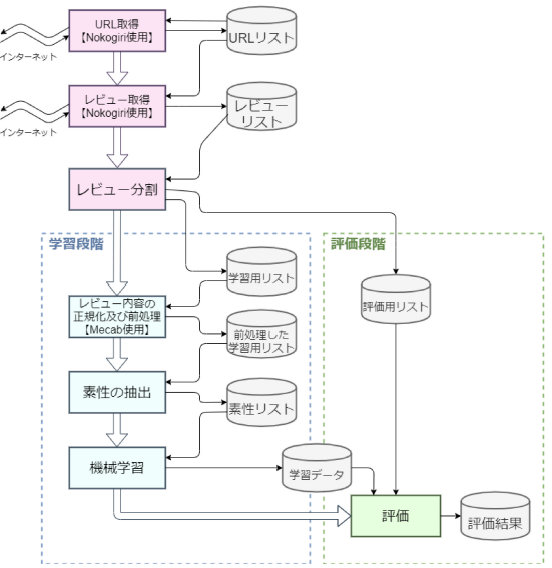
\includegraphics[width=10cm]{images/system1.png}
    \caption{システム概要図}
    \label{fig:関連研究1システム概要図}
\end{figure}
この研究はレビューを参考になる順序に並べ替えることが目的のため, 素性には単語の出現頻度を用いている. 
目的変数をレビューが参考になる確率$P$とし, 抽出した素性を用いてロジスティック回帰により学習する. 
ロジスティック回帰のモデル式は式(1)で示される. $\theta_i$は素性の重み, $N$は素性の数を表している. 
\vspace{5truept}

\begin{equation}
    P=\dfrac{1}{1+exp(\theta_0x_0+\theta_1x_1+\cdots+\theta_Nx_N)}
\end{equation}
\vspace{5truept}

次に学習したモデルを用いて, 評価用データに対して実験を行ない, 提案システムの精度を検証している. 
この研究の提案システムの精度の評価は, 実際の商品ページのレビューの並び順との一致率で評価している. 
正解の並び方を$L_R$, 提案システムによる並べ方を$L_P$としたとき, それぞれの要素の一致率を$P_{match}$としている. 
例えば, 以下の並び方のとき, $P_{match}=100\%$となり最も良い結果となる. 
\begin{align}
    L_R:\{1,2,3,4,5\}\notag\\
    L_P:\{1,2,3,4,5\}\notag
\end{align}
しかし, 以下のように並び方の評価としては良い結果と言える場合でも, 5件のレビュー中1件のみ一致していることになり, 
$P_{match}=20\%$と低い結果になる. 
\begin{align}
    L_R:\{1,2,3,4,5\}\notag\\
    L_P:\{4,1,2,3,5\}\notag
\end{align}

このように正しい評価が行えない場合を解決するため, この研究ではクイックソートを利用した新しい評価法のQE法(Quicksort Evaluation method)
を提案している. QE法ではピボットを中央値とし, 昇順にするために要素を入れ替えた回数$S_{count}$と, 要素数における最大の入れ替え回数
$S_{max}$を用いた式(2)により, 評価値$P_{QE}$を求めている. なお, $S_{max}$は全ての要素が逆順の場合にクイックソートで
昇順に入れ替えた回数である. 
\vspace{5truept}

\begin{equation}
    P_{QE}=1-\dfrac{S_{count}}{S_{max}}
\end{equation}
\vspace{5truept}

実際の商品レビュー52,403件を取得し, そのうち51,403件を学習用データ, 1,000件を評価用データに分けて実験を行い, 提案システムの
精度を評価した結果を表\ref{table:関連研究1結果}に示している. 
ここで, 登場回数$F$とは学習の素性とするか決定するための単語の出現回数である. 
表\ref{table:関連研究1結果}から, $F=5000$, 学習率$\eta=1.7$のときに評価値$P_{QE}=0.814$と最大になる. 従って, この論文で提案しているシステムは
レビューを参考になる順序に並び替える手法として有効であると言える. 

しかし, この論文ではAmazonの商品レビューを分析の対象としていて, 素性には単語の出現頻度を用いているため, 
提案システムが成り立つにはしっかり商品をレビューしている文章を学習させる必要がある. そのため, この論文で提案されているシステム
ではYouTubeで商品を宣伝している動画や, SNSの投稿に対するコメントを学習させた場合に上手く学習できなかったり, 精度が悪くなってしまう
ことが考えられる. なぜならば, YouTubeの動画やSNSの投稿に対するコメントというのは誰でも気軽にでき, 内容も自由であるため, 
商品のレビューのようなコメントの数がAmazonの商品レビューに比べると少ないからである. また, 一文の長さも短いことが多く, 素性となり得る単語の抽出
も難しいと考えられる. そこで, 本論文ではそのような問題を解決するための手法を第Ⅱ部で提案する.
\begin{table}
    \centering
    \caption{登場回数と学習率の組み合わせごとの評価値$P_{QE}$}
    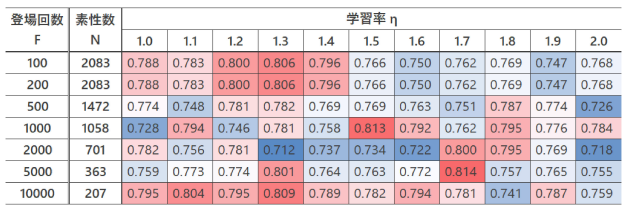
\includegraphics[width=14cm]{images/table1.png}
    \label{table:関連研究1結果}
\end{table}

\subsection{単語の出現頻度と類似性に基づいたトピックモデル洗練化手法[2]}
この論文では, 第Ⅱ部で後述するトピックモデルの一種のLatent Dirichlet Allocation(以下LDA)を自然言語文書に適用する際の
改善案を提案している. 
通常, トピックモデルを自然言語文書に適用する際には, 前処理として分類に不必要なストップワードの除去を行うことが多いが, 
一般的にストップワードリストに含まれている単語を除去するだけでは, 特定の文書にのみ頻出する特徴的な単語
を除去することが出来ず, トピックモデルの精度に影響を及ぼすという問題が存在する. 
また, トピックモデルによって分類したトピックには, 類似したトピックが複数出現し, 
分類の精度が下がるという問題も存在する. 

そこでこの論文では, 前処理として分析対象としている文書から適切なストップワードリストを作成する方法を提案している. 
また, トピックモデルを適用後の後処理として, トピックを構成している単語の類似度からトピック間の距離を算出し, 
類似しているトピックを統合することでより正確なトピック分類を可能にする手法を提案している. 図\ref{fig:関連研究2提案手法}は提案手法の全体像である. 
\begin{figure}[h]
    \centering
    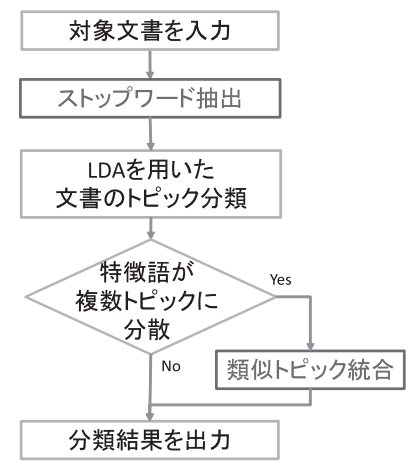
\includegraphics[]{images/fig2.png}
    \caption{提案手法の流れ}
    \label{fig:関連研究2提案手法}
\end{figure}

ストップワードリストを作成する手順を図\ref{fig:関連研究2ストップワード}で示している. この手法では, まず対象としている文書全体に対して出現率が高い
単語をストップワードとして抽出する. 出現率の算出にははDF(Document Frequency)を用いている. DFとは, 文書全体に対して
ある単語Tが含まれる文書数のことであり, 事前に設定した閾値よりも高いDF値を持つ単語をストップワードリストに加える. 
次に, 抽出した単語と意味的に類似している単語をさらにストップワードとしてリストに加える. 
word2vecを用いて文章中の各単語を周辺の単語から学習し, 単語の分散表現を得て単語間の類似度を算出する.  
それによりある単語Tの類似単語を抽出することができ, ある閾値以上の類似度を示した単語を全てストップワードリストに加える. 
これにより, DF値が高くない場合でも文書の特徴を表しにくい単語をストップワードリストに加えることが可能になる. 
\begin{figure}[h]
    \centering
    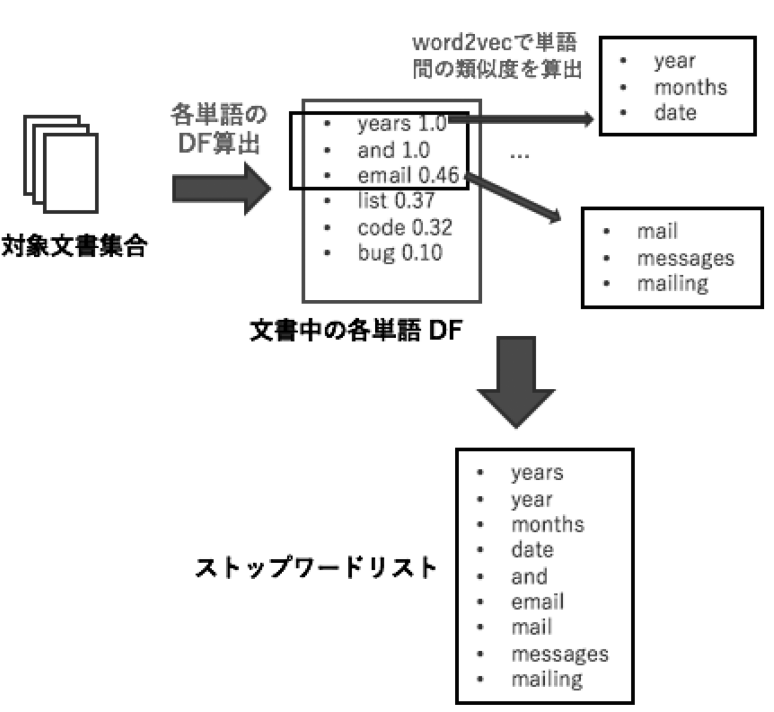
\includegraphics[]{images/fig3.png}
    \caption{ストップワード抽出手法の流れ}
    \label{fig:関連研究2ストップワード}
\end{figure}

トピックモデル適用後の後処理では, 分類結果に似たよったトピックが存在する場合にそれらのトピックを統合する処理を行うことを提案している. 
類似トピックの判断基準には, TF-IDF cos類似度推定法が用いられている. これは, cos類似度の計算に使用する
ベクトルの成分をTF-IDFで算出したものにした手法である. この研究では, 分類した各トピックの単語集合に対して
TF-IDF cos類似度を利用したクラスタリングを行い, その結果に従ってトピックを統合する手法を提案している. 

以上の提案手法をLDAのよるメーリングリストのトピック分類に適用し, 評価項目に基づいて比較することで提案手法
の有効性の評価を行っている. 評価項目として, 一般的なストップワードリストを用いた手法と提案手法を比較している. 
また, 後処理として類似トピックの統合を行った場合についても比較を行っている. 
トピック分類の正確さを評価する指標として, 適合率, 再現率, それらの調和平均のF値を採用している. 
実験結果を表\ref{table:関連研究2結果}に示している. 表\ref{table:関連研究2結果}より, LDAを自然言語に適用したトピック分類では, 前処理としてストップワード除去
を行うことで分類精度が大幅に向上していることが分かる. また, 一般的なストップワードリストを用いた場合と提案手法
によるストップワードリストを用いた方法を比較するとF値が向上している. また, 後処理を行った場合のF値はさらに向上している
ことから, トピック分類の正確性を向上させる提案手法の有効性を確認できている. 

本研究ではトピックモデルの分類精度よりも抽出する単語の質を重視しているため, この研究で提案されているストップワードリスト
作成方法を用いると抽出したい単語をストップワードリストに加えてしまう恐れがある. 
また, 本研究で分析の対象としているYouTubeのコメントは, 書き言葉よりも話し言葉で書かれていたり, 若者言葉が使われていることが多く, 
一般的なストップワードリストだけでは不要な単語を除去することが困難である. そのため, 前処理で形態素解析を行い, 特定の品詞のみ抽出
してストップワードとして除去する, または特定の品詞のみでトピック分類を行う手法で実験を行った. 
\begin{table}
    \centering
    \caption{ストップワード数($\#N$), 適合率, 再現率, F値の結果}
    \vspace{5truept}
    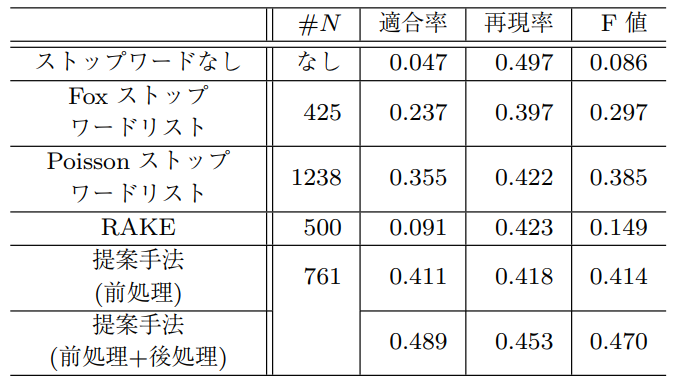
\includegraphics[]{images/table2.png}
    \label{table:関連研究2結果}
\end{table}

\subsection{関連研究3}
関連研究3 保留

\newpage
\section{研究目的}
前項までの関連研究を踏まえた上で, 本研究の研究目的を明らかにする. 本研究ではYouTube上で商品や
サービスを宣伝している動画に対する視聴者のコメントを分析対象とする. 対象としているコメントのうち, その動画で紹介している商品・
サービスと関連性が高いコメントを抽出するシステムの作成を目的としている. [1]でレビューを参考になる順序に並び替えているように, 
本研究では後述する提案手法により商品との関連性が高い順にコメントを並び替え, 他のユーザーがその商品の購入を検討する際に参考にするコメント
を取得しやすいシステムの作成を目指す. また, 作成したシステムにより抽出した商品との関連性が高いコメントが, 人手の評価に対してどれほどの精度
で抽出できているかを評価し, 最終的な提案手法の精度としている. 

\newpage
\part{提案手法}
第Ⅱ部では本研究の提案手法, 及び提案手法で用いている主要な技術について説明する. 
\section{トピックモデル}
提案手法の説明に先立ち, 本提案手法において主要な技術であるトピックモデルについて説明する. トピックモデルとは, 
%本読んでからがいい
\subsection{Latent Dirichlet Allocation}
LDAの説明
\subsection{Biterm Topic Model}
BTMの説明

\newpage
\section{提案手法}
ここでは, 前項で説明したBitem Topic Modelを用いて, YouTube上で自社製品やサービスを宣伝している動画
に対するユーザーのコメントから, 宣伝している商品やサービスに対して関連性が高いコメントを抽出する
システムを提案する. また, 提案したシステムの精度を検証する方法についても説明する. 
\subsection{データ収集}
実験に用いるYouTubeのコメントは, YouTube Data API v3を用いて取得した. YouTube Data API v3はGoogle Cloud Consoleで
APIキーを作成し, APIを有効化することで様々なYouTubeデータにアクセスすることが可能になる. 
そのうち, YouTubeのコメントに関連するものとして表\ref{table:データ収集}のようなデータが挙げられる. 
\begin{table}[h]
    \caption{YouTube Data API v3 で取得できるコメント情報}
    \vspace{5truept}

    \centering
    \begin{tabular}{ll}
        \hline
        項目 & 内容 \\
        \hline\hline
        videoID & コメントした動画のID\\
        textDisplay & 現在表示されているコメント\\
        textOriginal & 最初に投稿されているコメント\\
        authorDisplayName & コメント投稿者の名前\\
        authorProfileImageUrl & コメント投稿者のアイコン\\
        authorChannelUrl & コメント投稿者のチャンネル\\
        authorChannelId & コメント投稿者のチャンネルID\\
        likeCount & コメントに付いたいいねの数\\
        publishedAt & コメントの投稿日\\
        updatedAt & コメントの最終更新日\\
        \hline
    \end{tabular}
    \label{table:データ収集}
\end{table}

本研究では, 表\ref{table:データ収集}のうちtextDisplay(現在表示されているコメント)のみを抽出し, 実験を行なった. 
また, YouTubeのコメントには元のコメントの他に別のユーザーが返信しているケースも多いが, 本研究では返信しているコメントは扱わず, 
元のコメントのみを抽出し実験の対象としている. 抽出したコメントの一例を図\ref{fig:元コメント}に示す. 
\vspace{10truept}

\begin{figure}[h]
    \centering
    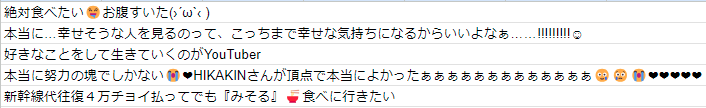
\includegraphics[width=14.5cm]{images/元コメント.png}
    \caption{抽出したコメントの一例}
    \label{fig:元コメント}
\end{figure}
\newpage

\subsection{前処理手法}
トピックモデルを含む自然言語処理の様々な手法において, テキストデータに対する前処理は非常に重要である. 
Webテキストを扱う場合にはHTMLタグやJavaScriptのコードが含まれることもあり, 前処理としてそのような
ノイズを除去する必要がある. また, 本研究ではYouTubeの動画に対するコメントをテキストデータとして扱うが, 
YouTubeのコメントやSNSの投稿には絵文字や顔文字, URL, 話し言葉などを含んでいることが多い. 
そのため, 本研究でもトピックモデルによる分類を行う前の前処理は非常に重要である. 
本研究で行った主な前処理とその簡単な説明を以下に示す. 
\vspace{10truept}

\subsubsection{クリーニング処理}
\begin{description}
    \item[空白、改行文字を削除]\mbox{}\\
    半角空白や全角空白, 及び``\textbackslash n"などの改行文字を空文字に変換する.\\
    例:「おはよう 今日はいい天気ですね」→「おはよう今日はいい天気ですね」
    \item[記号除去]\mbox{}\\
    ``!''や``\#'', 及び全角記号を除去する. また, YouTubeのコメントの特性上顔文字が使われることも多い
    ため, それらを除去する目的でもある. \\
    例:「今晩、友達と映画を見に行く予定です!楽しみですね( ˇωˇ )」→「今晩友達と映画を見に行く予定です楽しみですね」
    \item[絵文字除去]\mbox{}\\
    顔文字と同様にYouTubeのコメントで使われることが多い. 感情分析などでは絵文字から情報を取得することもあるが, 
    本研究では感情に関する情報の抽出, 分析は行わないため絵文字は除去する. 
    \item[数字を0に置換]\mbox{}\\
    自然言語処理の様々な手法において, 数字は意味を為さないことが多いため, 
    1つ以上連続している数字を全て0に置換することが多い. 本研究でも数字に関する情報を必要としないため, 
    数字はすべて0に置換する. \\
    例:「目標は年間で10回のイベントを開催することです」→「目標は年間で0回のイベントを開催することです」
    \item[単語の正規化]\mbox{}\\
    単語の正規化とは, 単語の文字種の統一, つづりや表記ゆれなどを無くすことである. この処理を行うことで
    同じ意味で異なる表記や形態の単語が同じ形になり, テキストの処理や解析が容易になる. 
    単語の正規化にはいくつか種類があり, 例えば
    \begin{itemize}
        \item テキスト内のアルファベットを全て小文字に変換する
        \item 半角カナを全角に統一する
        \item 辞書を用いた単語の統一
    \end{itemize}
    などがある. \\
    例:「Googleでネコの写真を検索してください」→「googleでネコの写真を検索してください」
    \newpage
    \item[連続長音記号除去, 繰り返し文字のまとめ]\mbox{}\\
    話し言葉や若者言葉でよくある「きたーーーーーー」や「うおおおおおお」など, 連続して長音記号が含まれている
    場合や同じ単語が繰り返されているものを削除, または一つにまとめる処理を行った. \\
    例:「食べたーーーーい!!」→「食べたーい」
    \item[その他の前処理]\mbox{}\\
    スパムの可能性があるため, URLを含むコメントを削除した. また, YouTubeの特性上外国人のコメントも多く存在したため, 
    日本語と英語以外の言語を含んでいるコメントを削除した. 
\end{description}

以上の前処理を図\ref{fig:元コメント}のコメントに適用した結果を図\ref{fig:前処理}に示す. 
\begin{figure}[h]
    \centering
    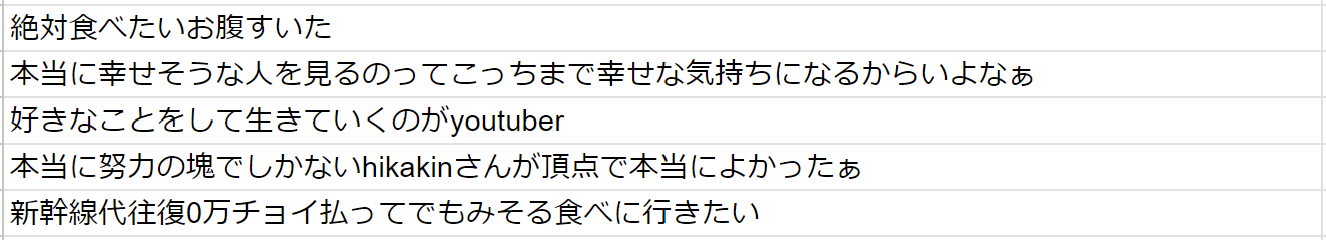
\includegraphics[width=14.5cm]{images/前処理適用.png}
    \caption{前処理後のコメント}
    \label{fig:前処理}
\end{figure}

\subsubsection{MeCabによる形態素解析及び分かち書き}
次に, トピックモデルで学習する際に必要な文章の分かち書きを行う. 分かち書きとは, 自然言語処理の様々な手法において
文章を単語や形態素などの最小単位に分割する処理のことである. この処理を行うことで, 言語解析や機械学習の際に
テキストをより扱いやすい形態で実験を行うことが出来る. また, 英文の場合は単語間にスペースが明示的に存在するため
分かち書きは必要ない場合が多いが, 日本語に関しては単語間のスペースがなく, 文章を単語単位に分割する処理を
行わないと機械が単語を認識し解析することが難しくなるため, 分かち書きが必要である. 

本研究ではMeCab[参考文献]を利用して形態素解析, 及び分かち書きを行った. MeCabは京都大学情報学研究科と
日本電信電話株式会社コミュニケーション科学基礎研究所の共同研究で開発されたオープンソースの日本語形態素解析エンジンであり, 
日本語の文法や単語の品詞情報をもとに文章を形態素に分解したり, 品詞の付与などが可能である. 
本研究ではMeCabを利用して対象のコメントに対して形態素解析を行い, 形態素に分割後スペース区切りで繋ぐことで分かち書きを行う. 
MeCabには最初から分かち書きを行う機能も含まれているが, 形態素解析によって抽出した品詞をストップワード除去に用いるため
この手法で分かち書きを行う. 
   
また, 形態素解析の精度はエンジンのアルゴリズムの精度に加え, 形態素解析辞書の精度にも左右される. 
そのため, 形態素解析の目的にあった辞書を指定し, 解析することが重要となる. 表\ref{table:辞書比較}はMeCabで形態素解析を行うときに主に用いられている
辞書を比較したものである. 通常, MeCabでの形態素解析には標準搭載されているmecab-ipadicを用いるが, mecab-ipadicは基本的な文法や
専門用語に強い反面, 辞書の更新がないため新しい単語や固有表現に弱いという特徴がある. 
本研究の分析対象であるYouTubeの動画に対するコメントは比較的新しい言葉や固有名詞などを含むことが多いため, 
mecab-ipadicに多数のweb上の言語資源から得た新語を追加し, カスタマイズしたmecab-ipadic-NEologdを本研究では形態素解析の辞書に用いている. 
\begin{table}[ht]
    \caption{形態素解析辞書の比較}
    \vspace{5truept}

    \centering
    \begin{tabular}{cp{10cm}}
        \hline
        形態素解析辞書 & 特徴 \\
        \hline\hline
        mecab-ipadic & IPAコーパスをもとにしたMeCabに標準搭載されているIPA辞書. 基本的な日本語の文法や専門用語などの固有名詞に強いが, 辞書の更新がないため新しい言葉や固有名詞に弱い. \\
        \hline
        UniDic-mecab & 言語学・国語学や音声情報処理など, より多様な目的に適した辞書. 「短単位」という揺れが少ない斉一な単位を見出し語に採用している. \\
        \hline
        mecab-ipadic-NEologd & 多数のweb上の言語資源から得た新語を追加しカスタマイズしたMeCab用のシステム辞書. 辞書の更新が行われるので, 新しい固有表現に強い. \\
        \hline
    \end{tabular}
    \label{table:辞書比較}
\end{table}
\newpage

MeCabによる形態素解析, 及び分かち書きの処理を行った後, 2.2節で述べた通り品詞によるストップワード除去を行う. さらに一般的なストップワードリストを
用いたストップワード除去を組み合わせることで, 最終的に実験に用いるテキストの形式として整形する. 品詞によるストップワード除去では, 助詞・助動詞
などのトピック分類に必要ない品詞を除く手法や, 名詞・形容詞などのトピックにかかわる品詞を抽出する手法で行う. 
図\ref{fig:形態素解析}ではmecab-ipadicとmecab-ipadic-NEologdで形態素解析した結果を比較している. 例えば, 近年登場した少年漫画である「鬼滅の刃」という単語を含む文章を形態素解析した場合, 
mecab-ipadicでは``鬼'' ``滅'' ``の'' ``刃''と分割されてしまっているが, 辞書の更新が行われるmecab-ipadic-NEologdでは
``鬼滅の刃''と一単語で認識されていて, 適切な形態素解析が行われていると言える. 
\vspace{10truept}

\begin{figure}[h]
    \centering
    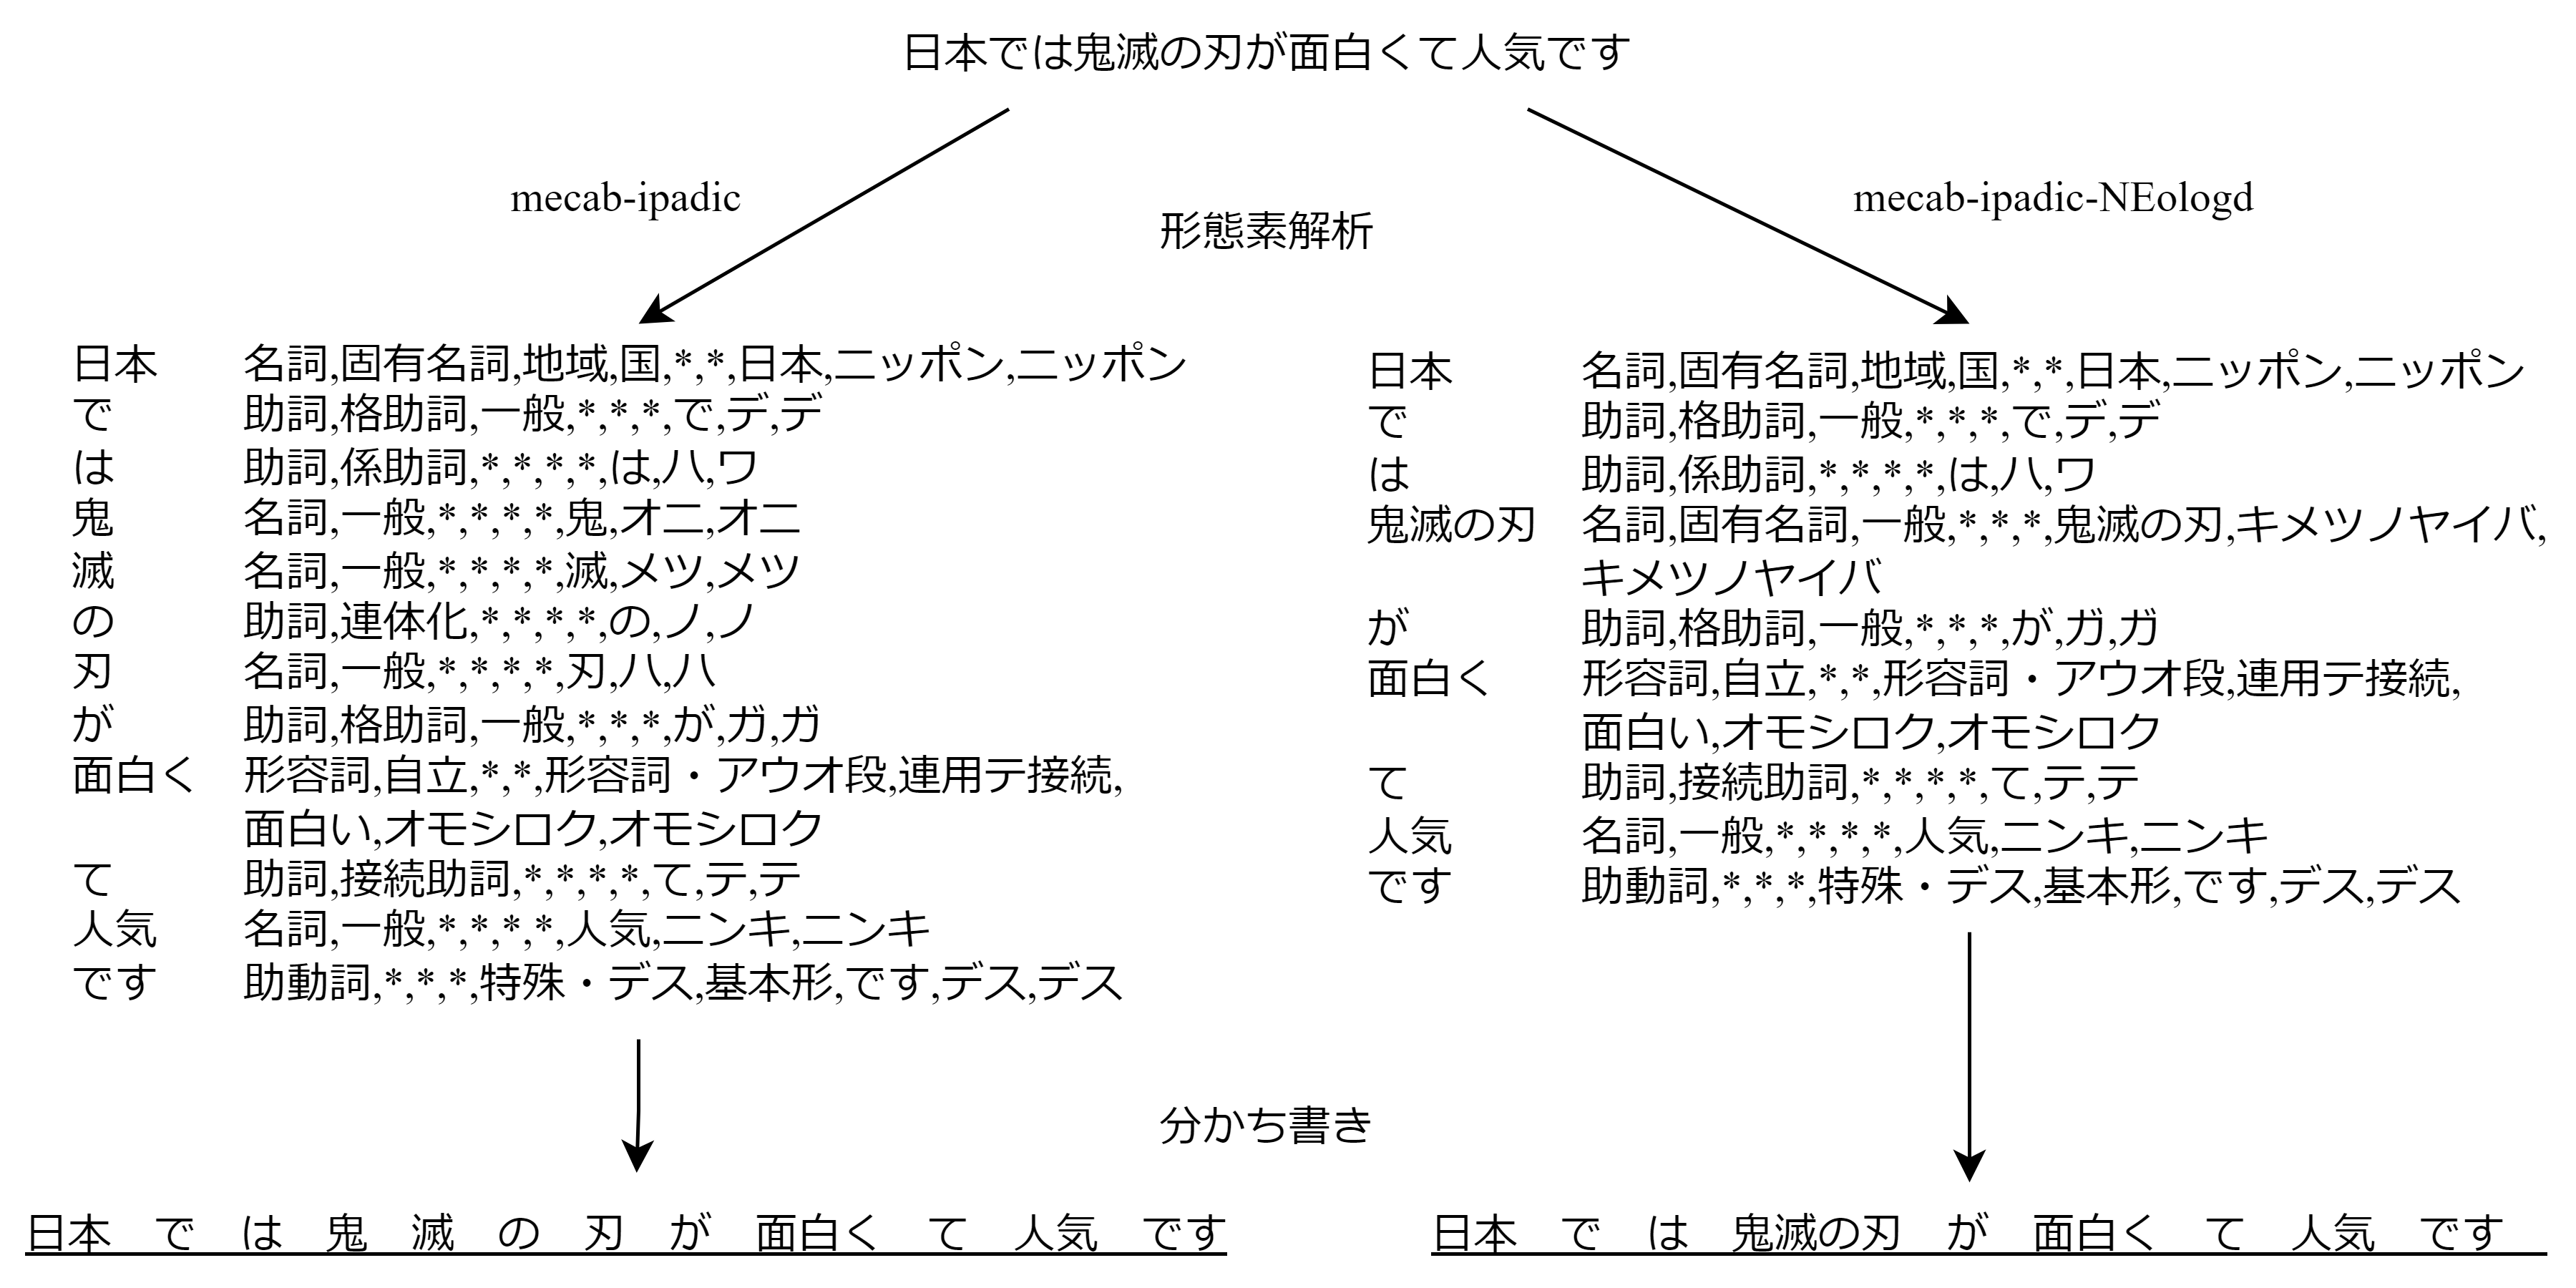
\includegraphics[width = 14.6cm]{images/形態素解析.drawio.png}
    \caption{辞書による形態素解析結果の比較}
    \label{fig:形態素解析}
\end{figure}

\newpage
\subsection{BTMによるトピック抽出}
%詳しい説明は4節でする
前処理及び分かち書きを行ったテキストデータに対し, 4.2節で説明したBiterm Topic Modelを適用する. 
BTMを適用することでテキストデータに存在する潜在的なトピックをハイパーパラメータで指定した数だけ推定し, 
トピックごとに出現しやすい単語を抽出する. 
%モデル、プログラムの説明、パラメータ

\subsection{文章生成}
次に, 各トピックごとの出現確率上位の単語を抽出した結果を用いて, 各トピックごとに文章を自動で生成する. 
抽出した単語は各トピックの出現確率上位の単語であるため, ここで生成された文章は各トピックごとに
代表的であるという仮説を立て, 以降の手法に適用する. 
文章を自動で生成する方法として, 大規模言語モデルであるGPT-3.5を搭載したChatGPTを用いる方法で行った. 
プロンプトには以下のルールを入力して各トピックごとに文章を生成した. 
\begin{description}
    \item[抽出した単語を空白区切りで入力する]\mbox{}\\
    BTMによって抽出したn単語(nは抽出する単語数)を空白区切りで入力する. ChatGPTに正しく単語を認識させるため, 
    空白区切りにする必要がある. 
    \item[全ての単語を使用しなくてもよい] \mbox{}\\
     抽出単語数によって長文が生成されることがあるため, 全ての単語を使う必要はない. 
    \item[人名がある場合は指定する]\mbox{}\\
    人名をChatGPTが認識できない場合, 文章が支離滅裂になる可能性があるため個別に指定する. 
    \item[一つの文章に多くの単語を用いて, 文章数は少なくする]\mbox{}\\  
    生成される文章はトピックごとに代表的であるという仮説の元, YouTubeのコメントの特徴に近い
    文章を生成したいため, 長文を避けるようなルールを追加している. 
\end{description}
図\ref{fig:文章生成}に入力する単語数, プロンプト, 出力結果の例を示す. 
\begin{figure}[h]
    \centering
    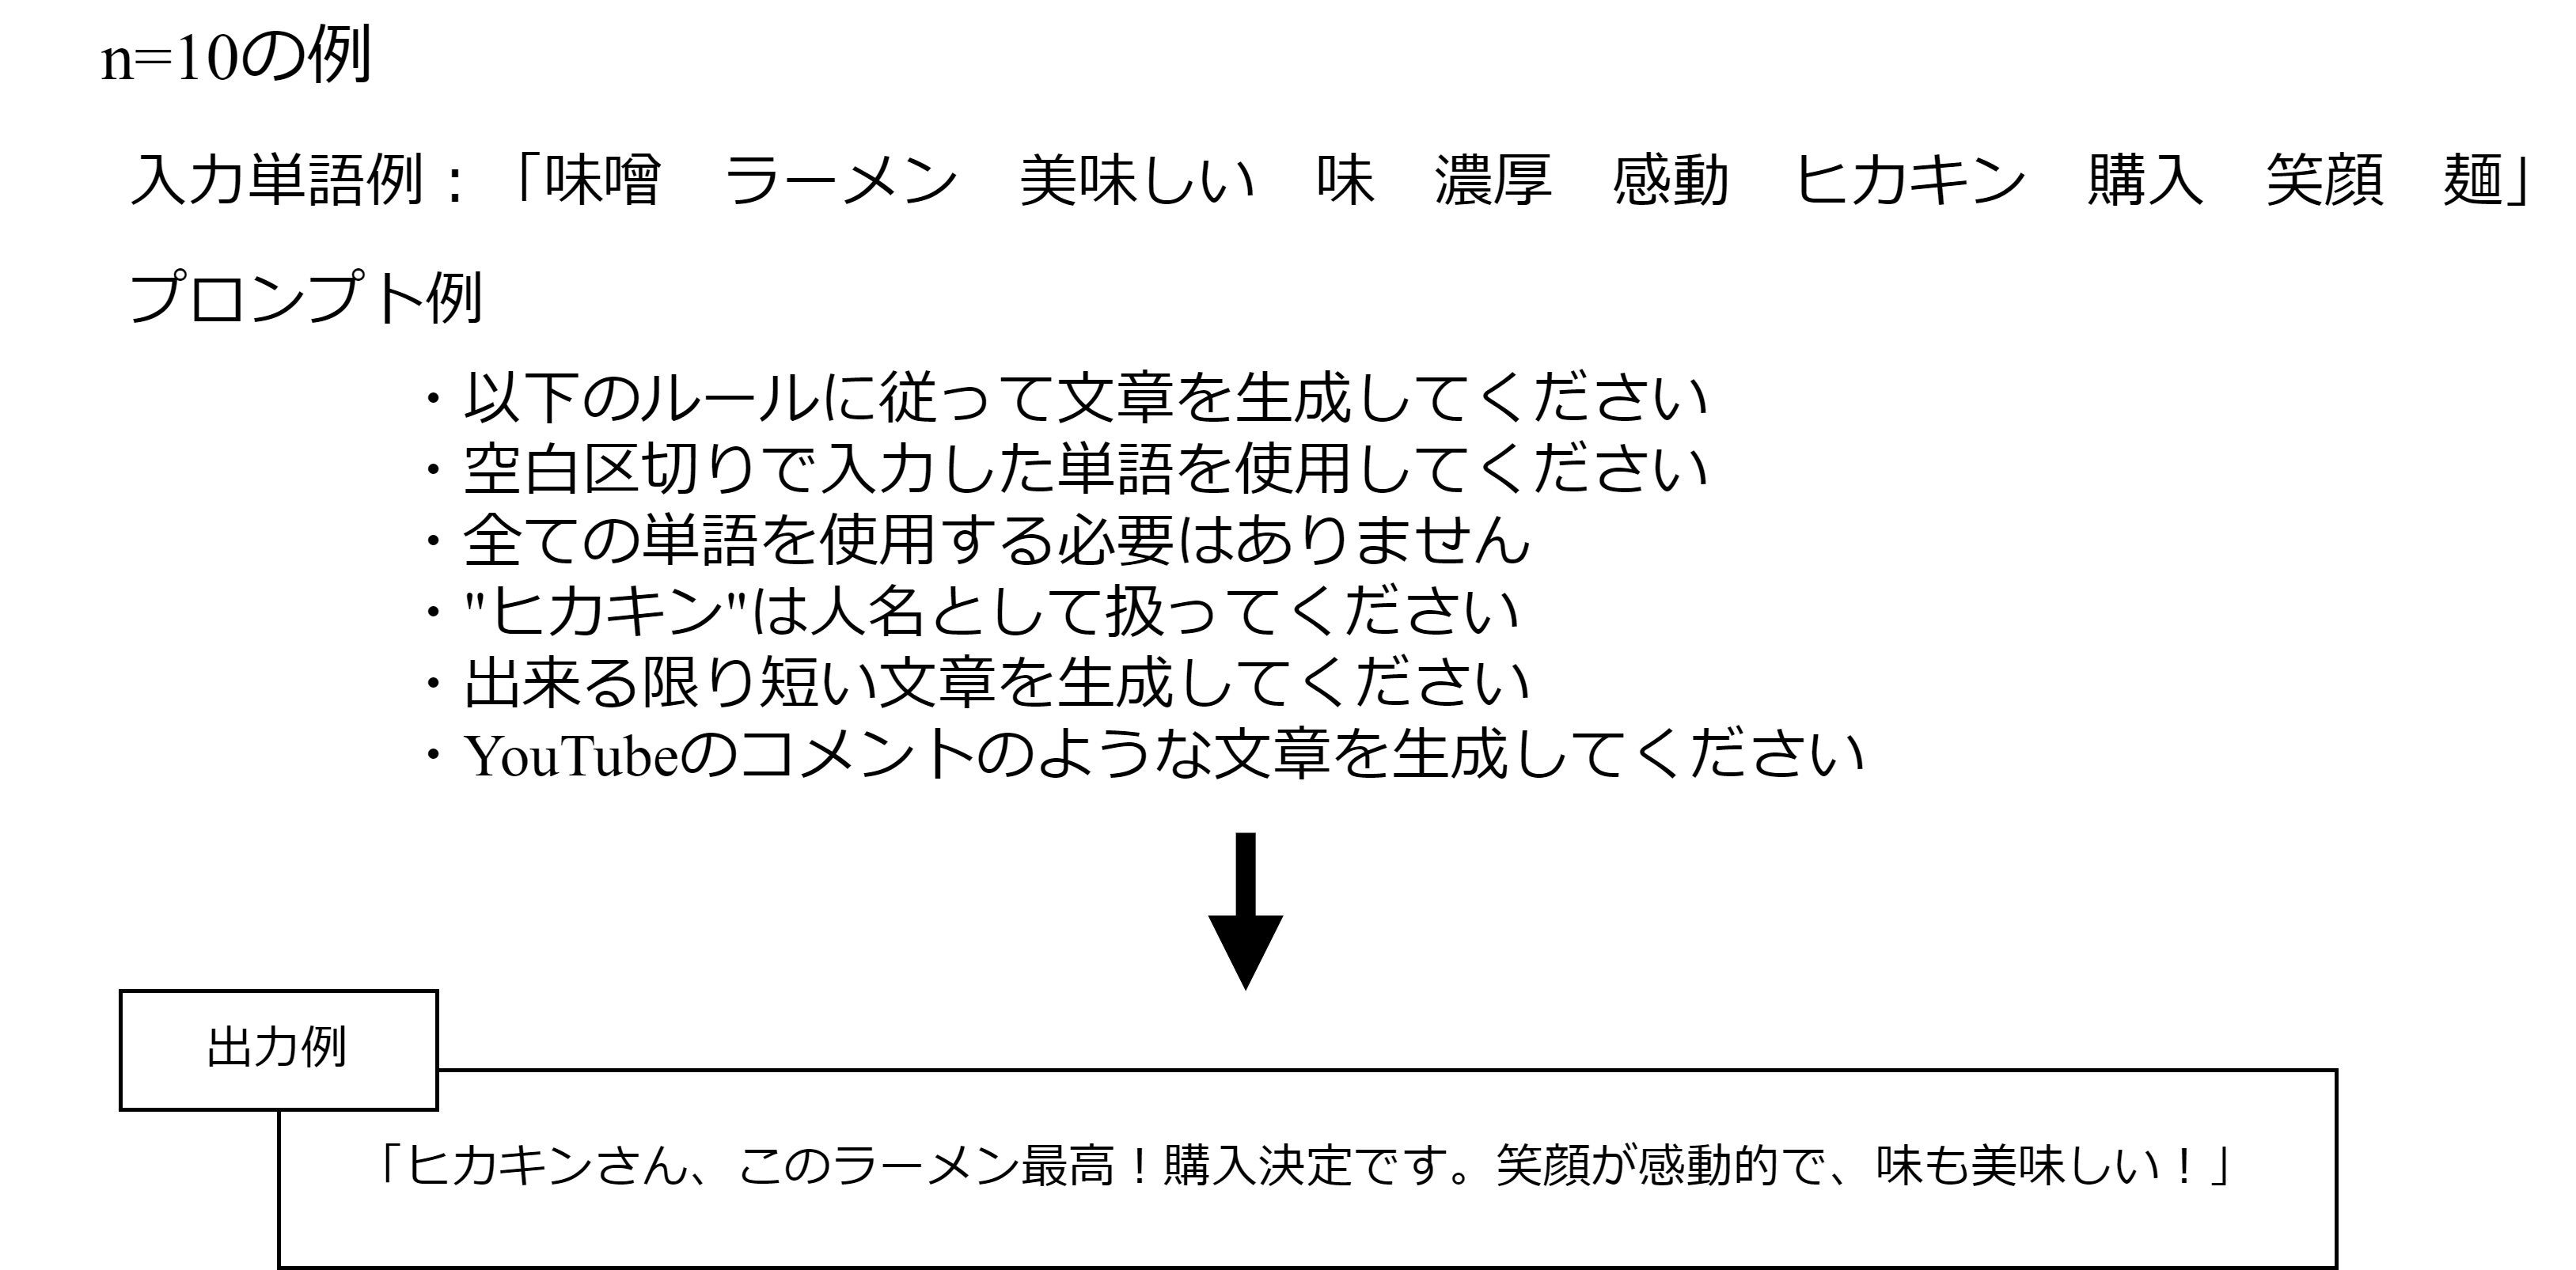
\includegraphics[]{images/文章生成.drawio.png}
    \caption{chatGPTを用いた文章生成}
    \label{fig:文章生成}
\end{figure}

\subsection{文章間の類似度計算}
%生成した文章の結果、元の文章との類似度、5文で一番高いのを採用
\subsection{提案手法の精度検証}
%元のコメントをアノテーション、基準、類似度上位との一致度計算、精度、正解率、F値の結果

\newpage
\part{実験結果}
\section{実験目的、仮説}
\part{参考文献}
[1]機械学習を用いた自然言語処理による商品レビューの評価

[2]単語の出現頻度と類似性に基づいたトピックモデル洗練化手法
\end{document}